\documentclass{article}
\usepackage[utf8]{inputenc}
\usepackage{amsmath,amssymb}
\usepackage{amsfonts}
\usepackage{paralist}
\usepackage{color}
\usepackage[table]{xcolor}
\usepackage{graphicx}
\usepackage{pgfplots}
\usepackage{authblk}
\usepackage{url}
\usepackage{multirow}
\usepackage{booktabs}
\usepackage{blindtext}
\usepackage{adjustbox}
\usepackage{subcaption}
\usepackage[margin=1.3in]{geometry}

\usepackage{float}
\usepackage[font=small, labelfont=bf, textfont=it, format=hang]{caption}
\usepackage[colorlinks=true, allcolors=blue]{hyperref}
\urlstyle{same}
\usepackage[english,nameinlink]{cleveref}
\usepackage{natbib} 
\crefname{equation}{}{}

\title{HPC Final Project}
\author{Valentinis Alessio [SM3800008]}
\date{27/02/2024}

\begin{document}
	\maketitle
	\tableofcontents
	
	\part{Exercise 1}
	
	The goal of the exercise is to estimate the latency of default openMPI implementation of two collective blocking algorithms, one of which being \textit{broadcast}, varying the virtual topology with which the algorithms operate, along with the map by whcich the cores are allocated.
	My choice resided into:
	\begin{itemize}
		\item \textbf{Broadcast}: varying algorithms among \textit{default}, \textit{basic linear}, \textit{flat chain} and \textit{binary tree}.\\
		\item \textbf{Barrier}: varying algorithms among \textit{default}, \textit{basic linear}, \textit{double ring} and \textit{bruck}.
	\end{itemize}
	
	The benchmark library used is OSU microbenchmark, available \href{https://mvapich.cse.ohio-state.edu/benchmarks/}{here}.
	The tests were conducted on the EPYC nodes in the ORFEO clusters and all tests were performed following a \textit{bash} script to automatize the process of data gathering.
	
	\section{Broadcast operation}
	
	MPI\_Broadcast is a fundamental collective communication operation provided by the Message Passing Interface (MPI) library. It allows one process, typically referred to as the root process, to efficiently broadcast data to all other processes in a communicator. This operation is crucial for distributing information across multiple processes in parallel computing environments. It's a widely used one-to-all operation that by default is implemented in multiple ways, in order to optimize the times taken for sending data to multiple processes.
	I will go into some further details only of those operations which are covered in this study.
	\begin{itemize}
		\item Default: this kind of implementation should authomatically choose the optimal way of sending the information, based on both size of the message and number of cores.\\
		\item Basic linear: it's the way we could think to naiively implement the broadcast algorithm, i.e. the root process sends sequentially to all processes the message, one by one.\\
		\item Chain: In this implementation, as the name suggests, the message is sent from one process to the other, so process0 sends its message to process1, process1 to process2, and so on and so forth.\\
		\item Binary tree: this virtual topology of the cores is such that they are organized in a binary tree fashion, so process0 is in charge of sending the message to process1 and process2, process1 to process3 and process4, and so on.
	\end{itemize}
	
	For some of these operations message segmentation is enabled, i.e. the message is divided in chunks, and these chunks are sequentially sent to the other processes. In particular we are referring to binary tree and chain.
	
	\subsection{Data collecting process}
	The process of collecting data has been authomatized through the use of a bash script, available in the GitHub repository \cite{repo}. 
	To have a better view of the what happens with different mappings of the cores, the same gathering process has been brougth on varying the \textit{--map-by} parameter, and to collect as many data in one shot, the maximum message has been truncated to 2024 bytes, which is anyway well beyond the latency-dominated size region.
	To allow for a better data gathering process, the different mapping of the processes (by core, by socket and by node), the different scripts have been separated.
	
	As previously announced, the tests have been brought up into the EPYC nodes, selecting and prioritizing the acces to two whole nodes. So, due to the characteristics of the computing architecture, I have conduced the test onto a maximum of 256 cores, distributed in four sockets and two nodes.
	
	To have better quality of the data collected, I chose to set 100 warmup operation and 10000 effective operations, from which the average has been taken and recorded.
	
	\subsection{Latency analysis}
	
	The data collection process generated a pretty substantial dataset, providing different combinations for algorithm, cores allocation and message size to analyze the average latency of the communication.
	To tackle this complexity and various combinations, my effort was to sequentially fix some degrees of freedom, while varying the others, one or more at the time. At the end I tried to develop a model that could explain the interaction between the various covariates and the Average Latency measurements.
	
	\subsubsection{Fix algorithm and vary allocation}
	
	In this part we explore the behavior of the various algorithm, for data size of 1 MPI\_CHAR, so 1 byte, by varying the number of cores and their allocation. This choice of the message size isolates and examines the "pure" latency of the communication.
	
	% INSERIRE IMMAGINE DI ALGORITMI PER 1 CHAR communications
	% 1a default
	% 1b linear
	% 1c chain
	% 1d binary
	
	\begin{figure}[h]
		\centering
		\begin{subfigure}{0.45\textwidth}
		\centering
		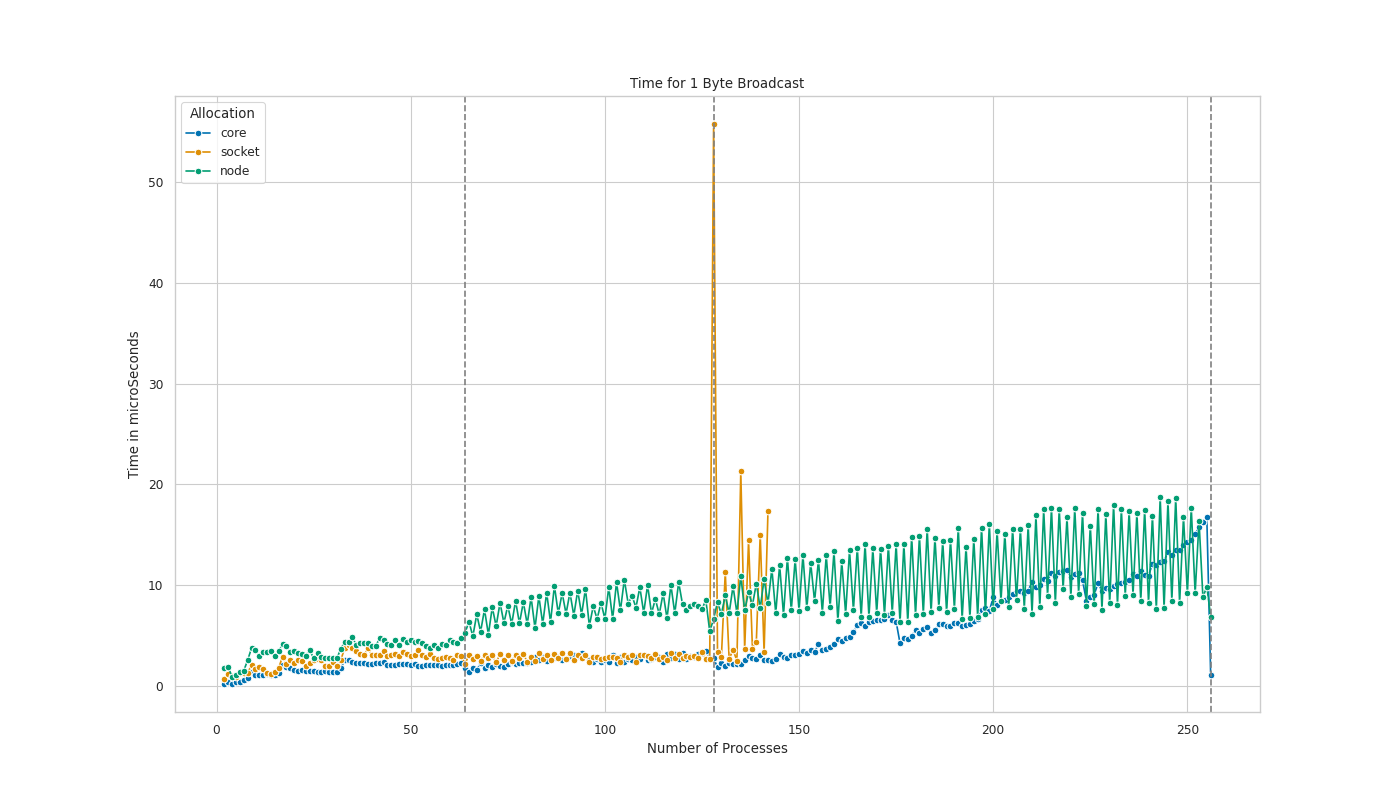
\includegraphics[width=0.7\linewidth]{../exercise1/plots/bcast_default_1byte}
		\caption{Average Latency vs n. processes in default algorithm}
		\label{fig:bcastdefault1byte}
		\end{subfigure}
		\begin{subfigure}{0.45\textwidth}
			\centering
			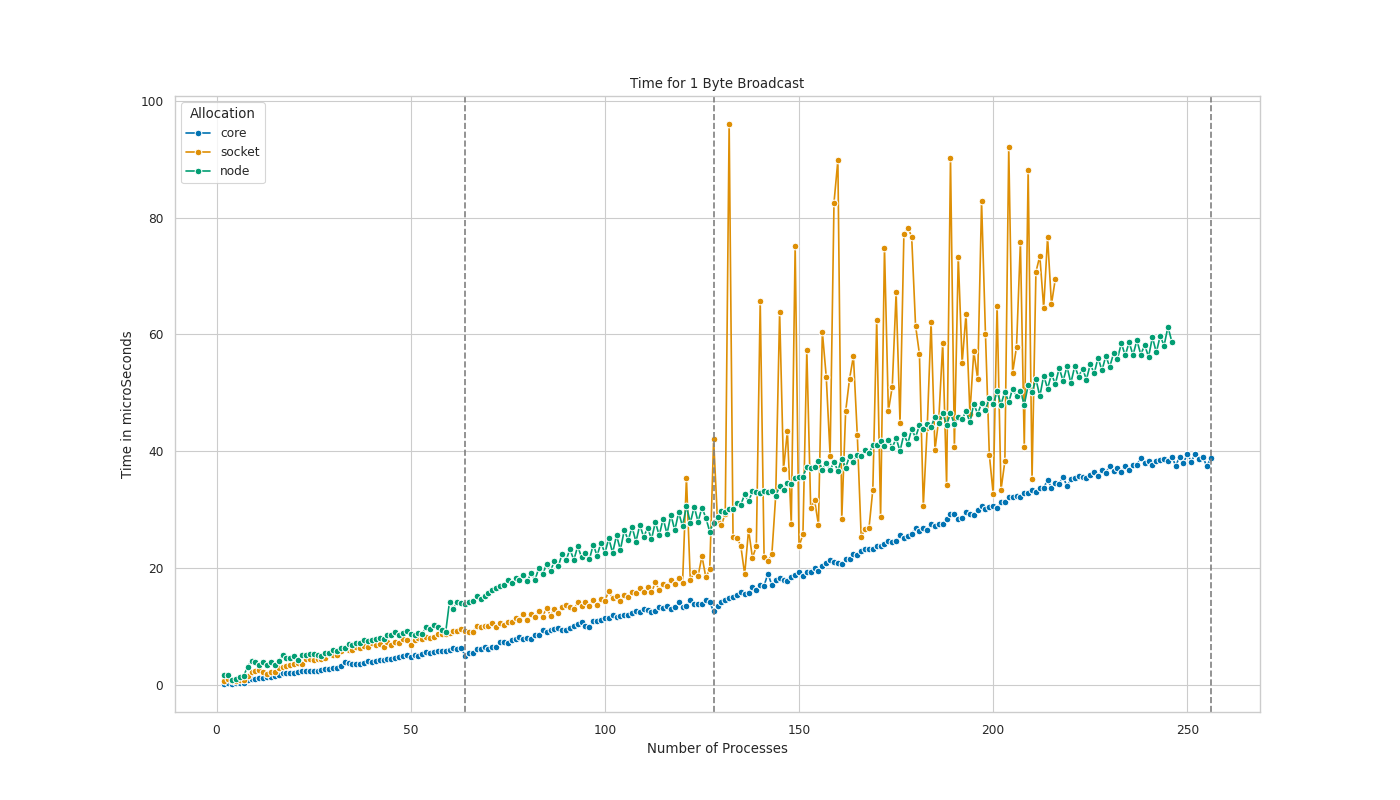
\includegraphics[width=0.7\linewidth]{../exercise1/plots/bcast_linear_1byte}
			\caption{Average Latency vs n. processes in linear algorithm}
			\label{fig:bcastlinear1byte}
		\end{subfigure}
		\begin{subfigure}{0.45\textwidth}
			\centering
			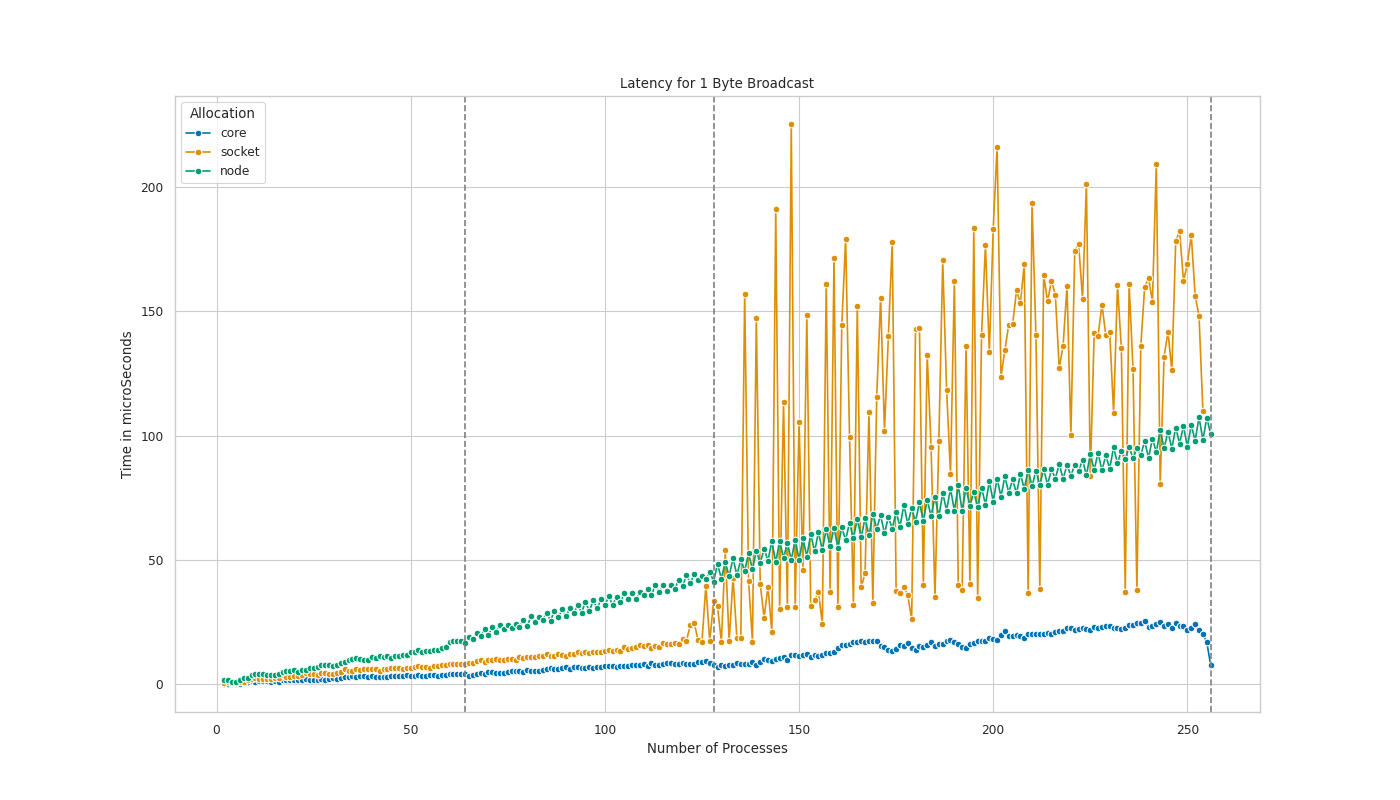
\includegraphics[width=0.7\linewidth]{../exercise1/plots/bcast_chain_1byte}
			\caption{Average Latency vs n. processes in chain algorithm}
			\label{fig:bcastchain1byte}
		\end{subfigure}
		\begin{subfigure}{0.45\textwidth}
			\centering
			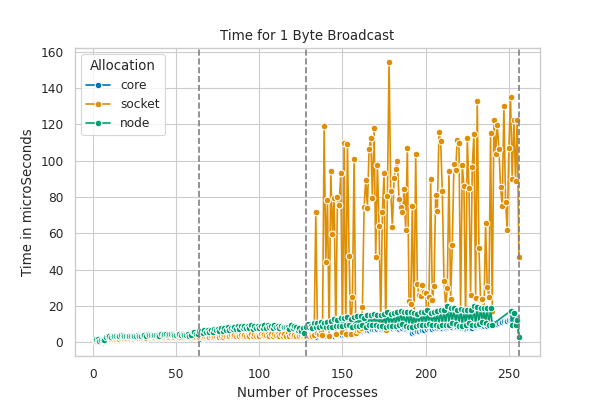
\includegraphics[width=0.7\linewidth]{../exercise1/plots/bcast_bintree_1byte}
			\caption{Average Latency vs n. processes in binary tree algorithm}
			\label{fig:bcastbintree1byte}
		\end{subfigure}
	\end{figure}
	
	
	
	Concerning the first plot, default algorithm behaves as expected, as we can clearly identify three regions, above all in core and socket mappings, with two noticable jumps and changing in behavior, while node allocation doesn't show remarkable and noticable jumps. The two jumps happen almost where expected, so at 64 cores, when we change socket, and at 128 cores, when we completely change node. It's worth to notice that the jump at the change of socket is by far more accentuated in the core mapping, as in that scenario cores are allocated as close as possible in the same socket. 
	
	Passing at the second plot, regarding the basic linear algorithm, we can observe almost the same behaviour at least for the core and node mapping. In socket mapping we can see that the change of behavior doesn't happen exactly at 128 cores as expexted, suggesting some more complicated model beyond "naive" node/socket changes.
	
	Going to the chain algorithm some similar observations to the previous ones hold, but with some peculiarities.
	In fact, differently from the previous ones, we can see the "serial" nature of the comunication, as the different positioning of the processes deeply impact on the latency measurements, with the node allocation by far diverging from the other two, at least in the one-node situation.
	
	Lastly, going to the binary tree algorithm, the lower latency measurements underscore and emphasize its (expected) superiority compared to the other algorithms. Moreover, we can see that allocating processes by node, we obtain some more stable latency when surpassing the 128 cores, showing some kind of optimized communication when dealing with processes inside the same node.
	Allocating by core or socket, instead, shows some jumps followed by immediate decreases in latency corresponding to the "region change" thresholds, which explanation may reside inside the hierarchical nature of the algorithm. In fact these phenomena could be due to the transition between two different levels of the tree, that may introduce some delay in the communication. Once this transition is passed, the latency decreases, as the subsequent level of the tree gets filled.
	
	\subsubsection{Compare algorithms fixing allocation}
	
	In this second part of our analysis, I fixed the allocation type to \textit{core}, as it shows all the expected changes in behavior, and is the less influenced by eventual iner-node traffic with other communication. Fixing this degree of freedom, I chose once more to analyze the 1 byte scenario, to isolate the pure latency of the communication, and varying number of cores and type of algorithm.
	
	% INSERT IMAGE OF ALL MAP BY CORE
	\begin{figure}[h]
		\centering
		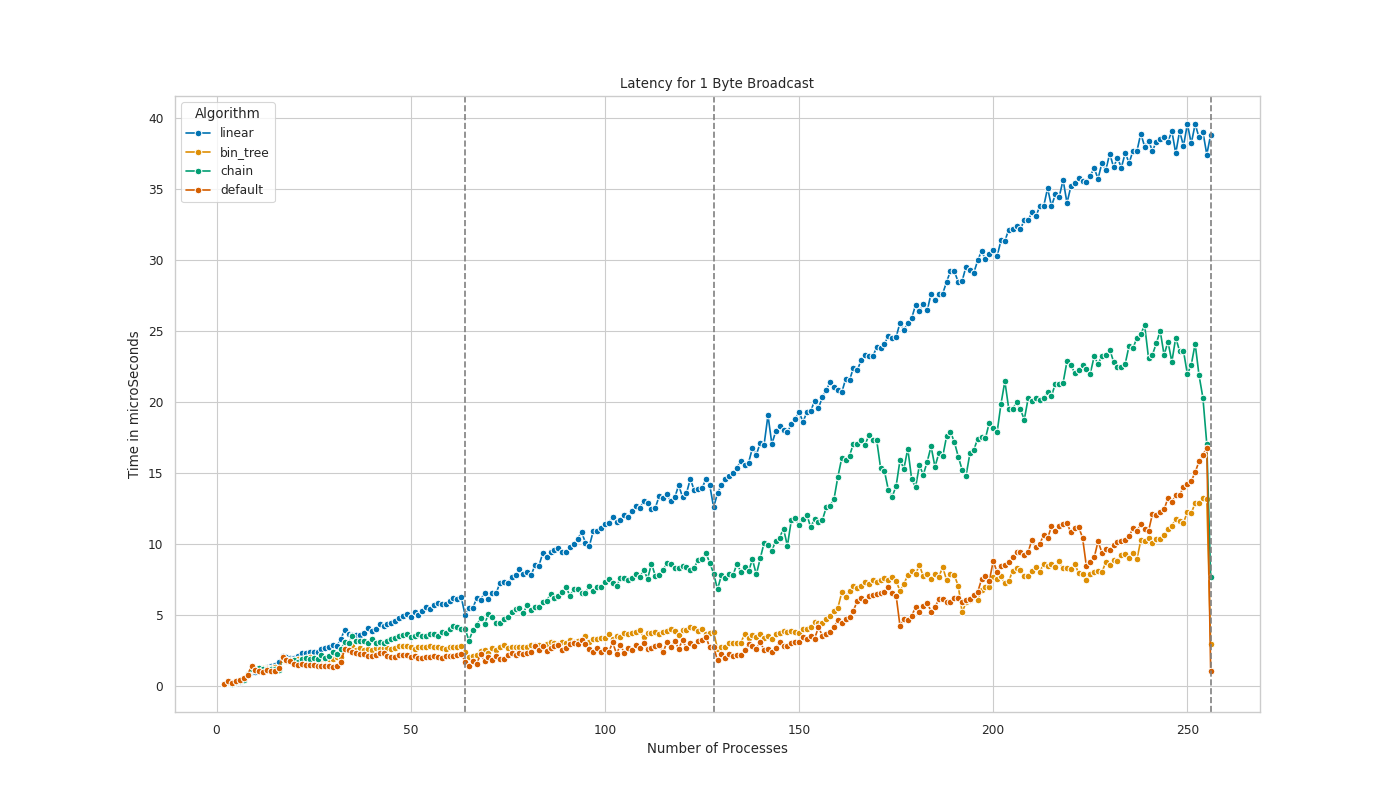
\includegraphics[width=0.7\linewidth]{../exercise1/plots/bcast_all_1byte}
		\caption{Latency vs n. processes by algorithm}
		\label{fig:bcastall1byte}
	\end{figure}
	
	
	The figure above offer some insights into how the algorithm influences the latency across three main regions:
	
	\begin{itemize}
		\item \textbf{Within 64 cores}: in this intra-socket region we can observe almost identical performances, which can be indicative of some optimal speed of communication occuring between cores in the same socket. The slight advantage observed with respect to the default and binary tree algorithm may be due to the fact that the first selects the send policy authomatically, while the latter organizes in a more optimal way the hierarchy of communication.\\
		\item \textbf{From 64 to 128 cores}: in this intra-node region we can begin to observe some more consistent advantage in terms of latency of the two algorithm mentioned above, which suggests that in this situation a choice among implementation may be done.
		\item \textbf{Above 128 core}: in this region we enter inter-node communication, and we can clearly state that the performance of the linear algorithm gets worse and worse, suggesting that with more processes to manage, the binary tree algorithm gains more than something in terms of performance, as the communication is done by a hierarchy processes, and not by one to all.
	\end{itemize}

	\subsubsection{Fixing allocation and vary message size}
	
	In this section we plan to analyze the various performance models among different message size.
	
	% INSERT IMAGES ABOUT DIFFERENT MESSAGE SIZES
	\begin{figure}[h]
		\centering
		\begin{subfigure}{0.45\textwidth}
			\centering
			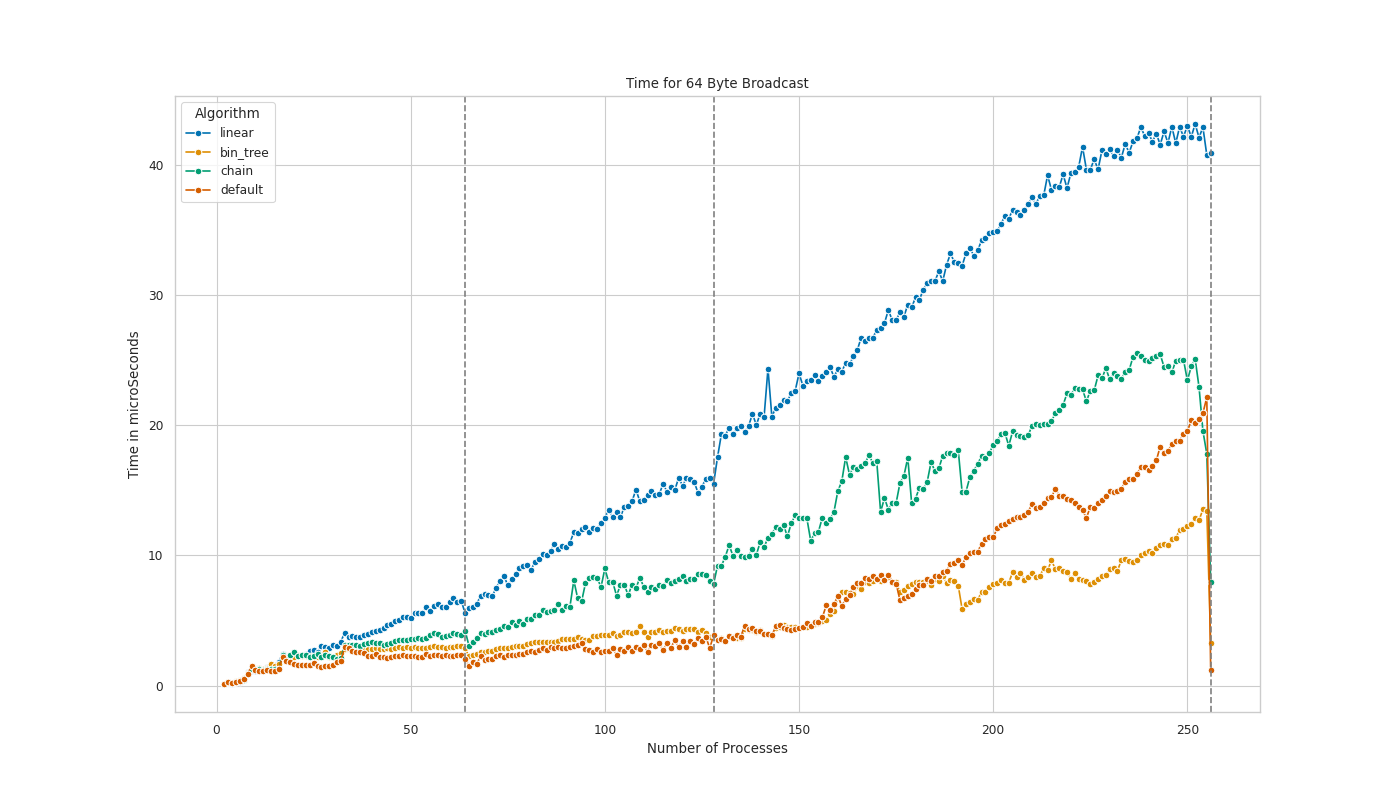
\includegraphics[width=0.7\linewidth]{../exercise1/plots/bcast_all_64byte}
			\caption{Average Latency vs n. processes for 64 byte message}
			\label{fig:bcastall64byte}
		\end{subfigure}
		\begin{subfigure}{0.45\textwidth}
			\centering
			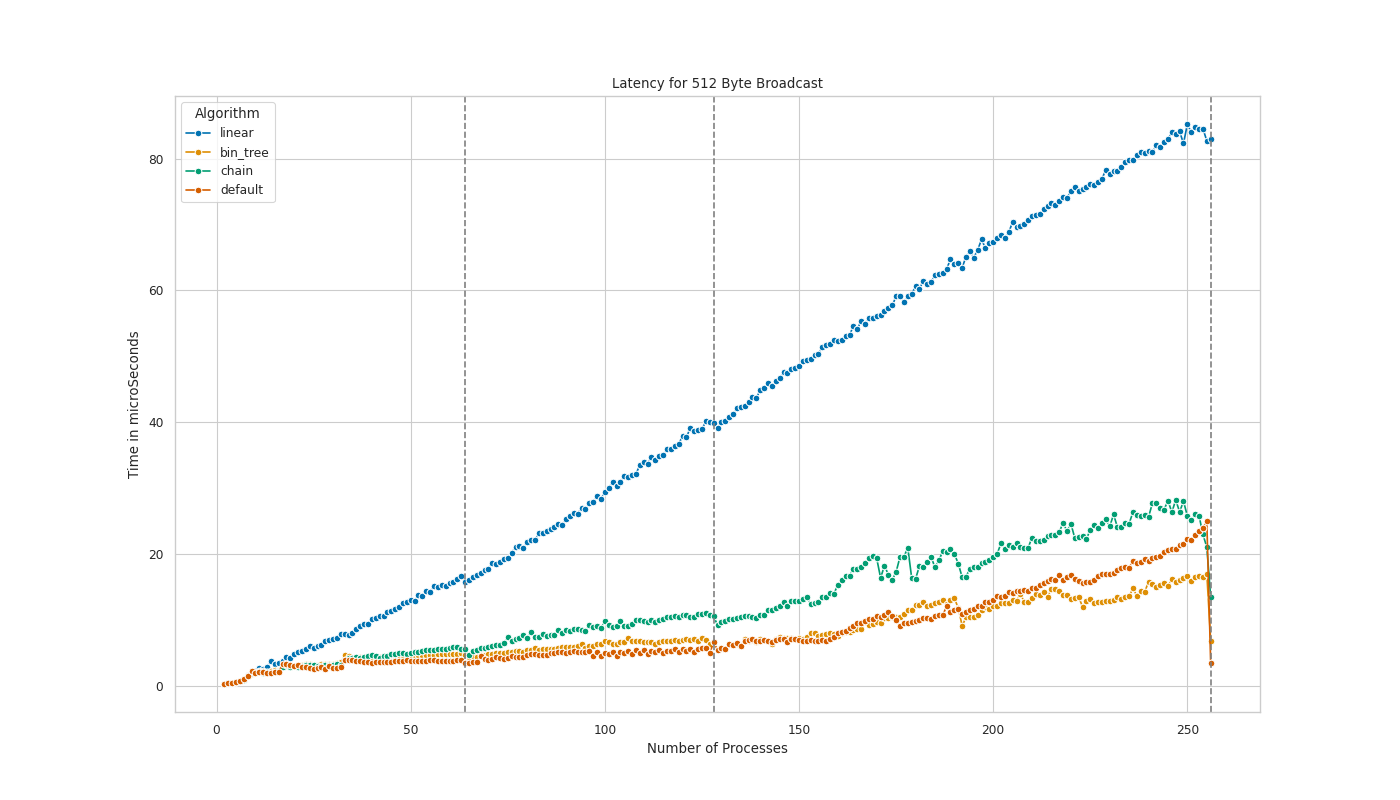
\includegraphics[width=0.7\linewidth]{../exercise1/plots/bcast_all_512byte}
			\caption{Average Latency vs n. processes in 512 byte message}
			\label{fig:bcastall512byte}
		\end{subfigure}
		\begin{subfigure}{0.45\textwidth}
			\centering
			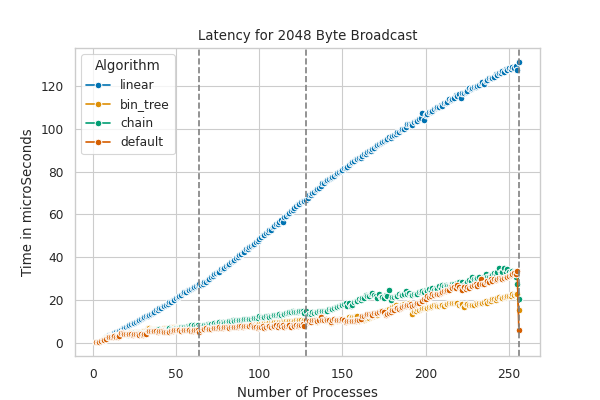
\includegraphics[width=0.7\linewidth]{../exercise1/plots/bcast_all_2048byte}
			\caption{Average Latency vs n. processes in 2024 byte message}
			\label{fig:bcastall2048byte}
		\end{subfigure}
	\end{figure}
	
	Varying message sizes we can observe more peculiar aspects of each implementations: while with a 1 byte message, the difference between implementations is pretty negligible as long we remain into the same node, varying message sizes, we can clearly see how the linear algorithm performs worse and worse increasing the message size.
	This behavior is due to two main factors: firstly the communication between processes is put as responsibility of the root process, which one by one sends the message to the other processes, while in all other algorithms the communication is organized in a more or less hierarchical way; secondly the linear approach is the only one among the analyzed ones that doesn't imply message segmentation, so in the linear algorithm the message is sent entirely from the root process to the remaining ones. The other methods, on the other hand, aside from the hierarchy of communications, allow for message segmentation, i.e. the message is divided in chunks and sent one chunk at the time via buffer-send (MPI\_ISend), as mentioned in the article suggested as reference \cite{bcast_article}.
	
	\subsection{Broadcast performance model}
	As a conclusive step of the analysis I attempted to formulate a performance model to try to better understand the not-so-straight-forward dynamics playing into these algorithms. 
	At firt I gave a try at estimating both latency and bandwidth within point-to-point communications employing again the OSU-microbenchmark library. The intention was to try and develop the Hockney model I found explained in some articles. However, the results obtained didn't fit well with the collected data, suggesting me to try something different. Maybe biased by my mathematical backgroud, or by some freshly sustained exams, I opted for the implementation of a linear model.
	
	With the use of the software R, my first attempt was to try and model the \textit{Average Latency} parameter on all the other parameters. This approach resulted not to be the most appropriate, other from the fact that not all the covariates resulted to be statistically relevant, such as, for example the \textit{Message Size} and the \textit{default algorithm}, the percentage of variability descripted by the model, represented form the $R^2$ coefficient, resulted to be less than $3\%$.
	This result is another evidence towards the fact that the Average Latency is not the actual linear combination between allocation, algorithm, message size and number of processors.
	
	% latex table generated in R 4.3.1 by xtable 1.8-4 package
% Wed Feb 14 17:42:34 2024
\begin{tabular}{rrrrr}
  \hline
 & Estimate & Std. Error & t value & Pr($>$$|$t$|$) \\ 
  \hline
(Intercept) & -68.0031 & 5.0067 & -13.58 & 0.0000 \\ 
  Algorithmchain & 48.3330 & 4.5653 & 10.59 & 0.0000 \\ 
  Algorithmdefault & 4.7424 & 4.5774 & 1.04 & 0.3002 \\ 
  Algorithmlinear & 12.0579 & 4.6361 & 2.60 & 0.0093 \\ 
  Allocationnode & 39.0153 & 3.9529 & 9.87 & 0.0000 \\ 
  Allocationsocket & 63.3617 & 3.9943 & 15.86 & 0.0000 \\ 
  Processes & 0.5054 & 0.0225 & 22.49 & 0.0000 \\ 
  MessageSize & 0.0013 & 0.0027 & 0.46 & 0.6452 \\ 
   \hline
\end{tabular}

	
	This suggested me to try and fit a spline polinomial refression, with the help of a GAM model. Despite the fact that the effective spline degrees of freedom for the \textit{Processes} variable resulted to be 8, so not at all linear, the Message Size, although continuing not to be statistically significant, resulted to have a linear effect on the \textit{Average Latency}.
	This model, although being far more complex and capable to capture some evident non linear  effects, resulted to be not more accurate than $3\%$, suggesting an even more intricated relationship between the variables.
	
	
	
	My last effort was to try and fix an allocation, to see if I would get more significant results.
	Fixing the allocation to \textit{core}, which as said above, showed a more smooth and predictable behavior, the results resulted to be much more sensible.
	In fact, starting from the statistic relevance of the variables, all of them showed a much lower p-value, included \textit{Message Size}, which before didn't seem to have an importance in estimating the Average Latency.
	Other from this aspect, the model was able to capture more than $65\%$ of the variability of the model, a value by far more relevant than the ones obtained before. This, although showing a sensible improvements in the esitimation of the Latency, clearly states that a simple linear model is able to capture little more than the majority of the variability. Anyway, the real model underlying the \textit{Average Latency} variable seems to have more complicated relations than a simple linear one, for example due to the virtual topology of the algorithm (think for example at the binary tree algorithm, which has $log_2$ operations with respect to the linear one).
	
	% latex table generated in R 4.3.1 by xtable 1.8-4 package
% Wed Feb 14 18:00:32 2024
\begin{tabular}{rrrrr}
  \hline
 & Estimate & Std. Error & t value & Pr($>$$|$t$|$) \\ 
  \hline
(Intercept) & -11.7242 & 0.2489 & -47.10 & 0.0000 \\ 
  Algorithmchain & 5.3313 & 0.2587 & 20.60 & 0.0000 \\ 
  Algorithmdefault & 0.5461 & 0.2587 & 2.11 & 0.0348 \\ 
  Algorithmlinear & 23.9312 & 0.2587 & 92.49 & 0.0000 \\ 
  Processes & 0.1198 & 0.0012 & 96.41 & 0.0000 \\ 
  MessageSize & 0.0080 & 0.0002 & 51.66 & 0.0000 \\ 
   \hline
\end{tabular}

	
	% INSERISCI PARTE RIGUARDO MODELLO LINEARE
	
	
	\section{Barrier operation}
	
	In this second part of the exercise, I chose to analyze and study the performance model of the MPI\_Barrier algorithm. It's an operation that allows for the synchronization of different process within the same communicator. It consists of a construct that guarantees that by the end of the operation, all the processes have at least entered it.
	This collective blocking operation becomes crucial when we want to synchronize the processes involved in some parts of our distributed program, to ensure coherent and predictable execution. Among the plethora of synchronization mechanisms, the barrier algorithm stands as a fundamental construct, enabling synchronization points within parallel programs.
	By default, the library OpenMPI offers different implementation of this algorithm, always characterized by peculiar virtual topology of the cores, or by different hierarchy of execution \cite{barrier_article}. In this study I have examined only four of the  several algorithms present.
	
	\begin{itemize}
		\item Default: this kind of implementation chooses authomatically the optimal way to synchronize the processes, based on their number and allocation.\\
		\item Linear: in this algorithm all nodes refer to a preselected root; once everyone has reported to the root, it sends a release message to everyone.\\
		\item Double Ring: in this algorithm, a zero-byte message is sent from a preselected root to its right circularly; a node can leave Barrier once it receives the message for the second time.\\
		\item Bruck algorithm: this implementation, alternatively from the two just descripted, which require $P$ communication steps, only requires $\lceil log_2P \rceil$. At a generic step $k$, process $r$ receives zero-byte message from and sends the same message to process $r - 2^k$ and $r + 2^k$ respectively. This process goes on untill each process have received the message from all other processes.
	\end{itemize}
	
	\subsection{Data collecting process}
	
	The process of collecting data, similarly to the first part, has been authomatized through the use of a bash script. To ensure a better all around view of the process, the same gathering process has been brought up on varying the \textit{--map-by} parameter. To allow the generation of a more complete dataset, the different scripts are divided, other than by algorithm, also by core mapping.
	
	As before, the tests have been conducted into the EPYC nodes, selecting two whole computing nodes fully reserved for this task.
	
	Similarly of what happened in the first part, to have more consistent and less biased data, I chose to select 100 warm up operations and 10000 effective misurations, from which the average has been taken and recorded.
	
	\subsection{Latency analysis}
	
	The data collection process generated a complete dataset, that can in principle allow for a quite extensive analysis. Similarly to the first part, my effort was to select and fix some degrees of freedom, while varying the others, and permitting for a simpler visualization of the data.
	At the end I tried to formulate a model that could explain the complex interaction between the various parameters.
	
	\subsubsection{Vary allocation for fixed algorithm}
	
	In this part we are going to explore the behavoiur of the various algorithms, by varying number of processes and their allocation.
	
	% INSERIRE IMMAGINE DI ALGORITMI PER 1 CHAR communications
	% 1a default
	% 1b linear
	% 1c ring
	% 1d bruck
	
	\begin{figure}[h]
		\centering
		\begin{subfigure}{0.45\textwidth}
			\centering
			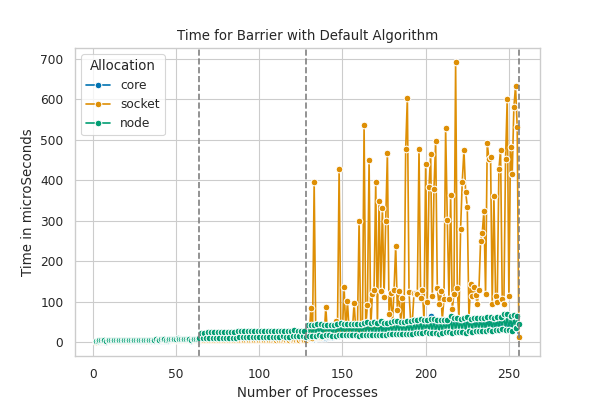
\includegraphics[width=0.7\linewidth]{../exercise1/plots/barrier_default}
			\caption{Average Latency vs n. processes in default algorithm}
			\label{fig:barrierdefault}
		\end{subfigure}
		\begin{subfigure}{0.45\textwidth}
			\centering
			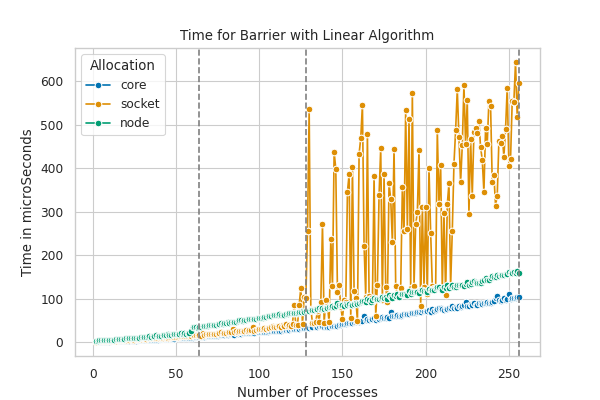
\includegraphics[width=0.7\linewidth]{../exercise1/plots/barrier_linear}
			\caption{Average Latency vs n. processes in linear algorithm}
			\label{fig:barrierlinear}
		\end{subfigure}
		\begin{subfigure}{0.45\textwidth}
			\centering
			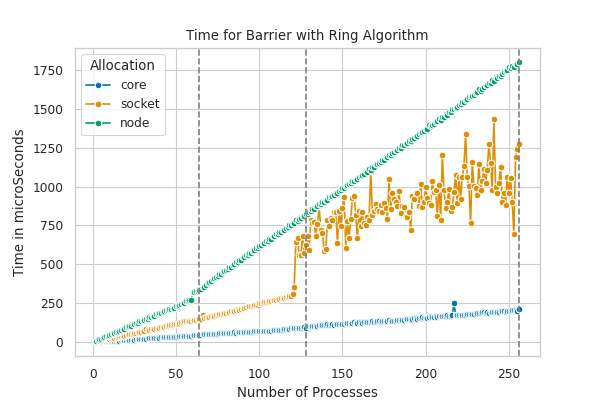
\includegraphics[width=0.7\linewidth]{../exercise1/plots/barrier_ring}
			\caption{Average Latency vs n. processes in double ring algorithm}
			\label{fig:barrierring}
		\end{subfigure}
		\begin{subfigure}{0.45\textwidth}
			\centering
			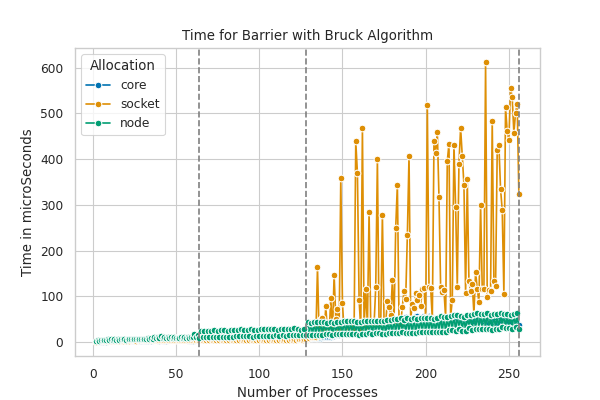
\includegraphics[width=0.7\linewidth]{../exercise1/plots/barrier_bruck}
			\caption{Average Latency vs n. processes in bruck algorithm}
			\label{fig:barrierbruck}
		\end{subfigure}
	\end{figure}
	
	Concerning the first plot we can clearly identify three different regions, one with less than 64 cores, where the three allocations seem to encounter the same latency, a secon up to 128 cores, where node allocations shows some worse behavior, and a third, when we exceed the number of processes into one node, where the socket allocation goes crazy while node distribution gains something with respect to core one. It's worth notice that, contrary to the broadcast algorithm, we cannot notice remarkable jumps in latency when we pass through some thresholds, as we are dealing with a zero-sized message communication among all processes.
	
	Passing to the second plot, regarding the linear algorithm, we can see almost the same characteristics as before, just with some more regular pattern into the node allocation. We can see that the changes in behavior don't happen where expected, suggesting some more complex interaction than the simple node/socket changes.
	
	Going to the Double Ring algorithm, we can see some pretty worse behavior in general, with higher values of the latency, and with clear separation between the three types of allocations. This may be due to the "serial" nature of the communication, where process0 waits for process1, which waits for process2, and so on and so forth untill each process receives the message for the second time. This reflects in an almost linear behavior in all the types of allocation, with the node distribution being from the beginning the worst one.
	
	Lastly, passing to the bruck algorithm, we can see some similar behavior to the default algorithm, with the same region division and almost the same behavior, suggesting that this algorithm may have an optimal hierarchy of communication, making it suitable for the default implementation.
	
	
	\subsubsection{Compare algorithms fixing allocation}
	
	In this second part of my analysis, I fixed the process allocation to \textit{core}, which showed to be more stable, other than being the least influenced by inter-node traffic.
	
	% INSERIRE IMMAGINE DI TUTTI GLI ALGORITMI MAPPATI PER CORE
	
	\begin{figure}[h]
		\centering
		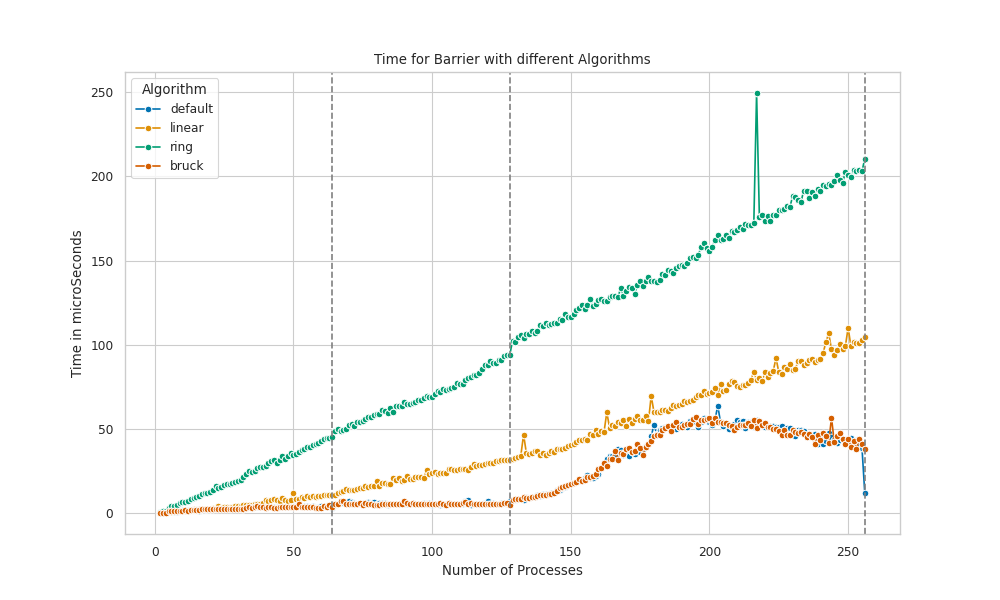
\includegraphics[width=0.7\linewidth]{../exercise1/plots/barrier_core}
		\caption{Latency vs n. processes by algorithm}
		\label{fig:barriercore}
	\end{figure}
	
	The figure above illustrates the four algorithms analyzed and offers some points of analysis straight away:
	
	\begin{itemize}
		\item Linear behaviors: we can clearly see as the double ring and linear algorithms have a quite consistent linear trend, justifying the linear number of communication required to complete the operation.
		\item Logarithmic trends: we can also see as the default and bruck implementation behave almost in the same way, suggesting that the latter is preferred. To justify the trend of the latency measurements, we have to take into consideration the bruck algorithm, where each process has to manage $log_2P$ Send operations. So within the same node we can see almost clearly the logarithmic behavior of the latency, while whe trepassing the node limit, due also to the inter-node latency in the communication, we have a "jump", and the same logarithmic trend reestablish when we have enough cores into the second node.
	\end{itemize}
	
	\subsection{Barrier performance model}
	
	Similar to the first part of the exercise, in this section my aim is to develop a statistical model that can explain the latency measurements as a function of the others degrees of freedom.
	
	Differently from the first part, here a simple linear model that included all covariates showed to have fairly good results.
	Analyzing statistical importance of the variables, we can state that all of them have a low p-value, except from the one related to the Default algorithm, which as we have seen from the qualitative analysis, almost perfectly mimics the bruck algorithm.
	As far as percentage of variability explained, I have obtained a $R^2=55\%$, which is a farly good result, but yet doesn't model all the complex variability of the underlying real model.
	
	% latex table generated in R 4.3.1 by xtable 1.8-4 package
% Wed Feb 14 17:58:54 2024
\begin{tabular}{rrrrr}
  \hline
 & Estimate & Std. Error & t value & Pr($>$$|$t$|$) \\ 
  \hline
(Intercept) & -68.0031 & 5.0067 & -13.58 & 0.0000 \\ 
  Algorithmchain & 48.3330 & 4.5653 & 10.59 & 0.0000 \\ 
  Algorithmdefault & 4.7424 & 4.5774 & 1.04 & 0.3002 \\ 
  Algorithmlinear & 12.0579 & 4.6361 & 2.60 & 0.0093 \\ 
  Allocationnode & 39.0153 & 3.9529 & 9.87 & 0.0000 \\ 
  Allocationsocket & 63.3617 & 3.9943 & 15.86 & 0.0000 \\ 
  Processes & 0.5054 & 0.0225 & 22.49 & 0.0000 \\ 
  MessageSize & 0.0013 & 0.0027 & 0.46 & 0.6452 \\ 
   \hline
\end{tabular}

	
	Similarly to the analysis conducted before, I chose to analyze also the single allocation case, focussing on the \textit{core} case.
	In this case, just considering the core allocation case, showed a considerable improvement in the model, showing similar statistical importance of the variables, but boosting the $R^2$ value to more than $80\%$. This shows how the barrier operation, instead of the broadcast one, has a "simpler" real model that regulates it, that can be fairly decently be estimated by a simple linear model.
	
	% latex table generated in R 4.3.1 by xtable 1.8-4 package
% Wed Feb 14 18:00:38 2024
\begin{tabular}{rrrrr}
  \hline
 & Estimate & Std. Error & t value & Pr($>$$|$t$|$) \\ 
  \hline
(Intercept) & -34.3959 & 1.5941 & -21.58 & 0.0000 \\ 
  Algorithmdefault & 0.0435 & 1.6956 & 0.03 & 0.9795 \\ 
  Algorithmlinear & 19.0073 & 1.6956 & 11.21 & 0.0000 \\ 
  Algorithmring & 78.4787 & 1.6956 & 46.28 & 0.0000 \\ 
  Processes & 0.4335 & 0.0081 & 53.23 & 0.0000 \\ 
   \hline
\end{tabular}

	
	% INSERIRE PARTE DI ANALISI STATISTICA
	
	\newpage
	
	\part{Exercise IIb}
	
	\section{Problem Statement: Parallel quicksort}
	
	The quicksort algorithm is the most known sorting algorithm used principally on arrays, based on the "divide and conquer" paradigm.
	It's core execution is divided in four parts:
	\begin{enumerate}
		\item Select a pivot;
		\item Partition the array around the pivot, putting the elements less than it in the first part, while the elements greater or equal to it, in the right part;
		\item \textbf{Recursive step}: Do this process recursively on the two halves of the array;
		\item \textbf{Base case}: when you have two elements in the array you are analyzing, swap their position if they are not ordered.
	\end{enumerate}
	
	\begin{figure}[h]
		\centering
		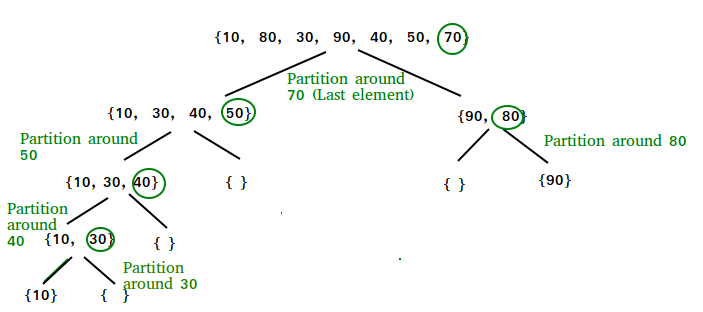
\includegraphics[width=0.7\linewidth]{QuickSort2}
		\caption[Illustration of Quicksort algorithm]{}
		\label{fig:quicksort2}
	\end{figure}
	
	
	In this exercise, the goal was to order a sequence of \textit{data\_t} elements, which are arrays of doubles with size 8, based on one of their elements, for simplicity let's say the first. All detailed informations about the assignment can be found at the referenced pdf \cite{ex2}.
	
	The aim of this project was to try and implement a parallel version of this algorithm using both MPI and OpenMP standards.
	
	\section{Implementation choices}
	Before starting to analyze implementation choices, a remark should be done in order to highlight a huge limitation of quicksort algorithm: by its nature it's not balanced, i.e. based on the choice of the pivot, the two recursions of the algorithm may have very different sizes. In some parts I tried some tricks to avoid this, but yet my solution is still far from optimal.
	Timings will cover only the ordering part, not considering the random number generation.
	
	\subsection{OpenMP}
	Regarding the OMP implementation, the only smart way I've come up for using multi-threading was on the recursion itself, in particular by spawning one task for each recursive call. This approach tries to parallelize two or more partition steps (which is the only thing the algorithm actually does). Of course this choice doesn't fully exploit the parallel power of a multithreading approach, as the optimal number of threads will not be the maximum achievable, but will strongly depend from the problem size, as for too little sizes, spawning more threads will only introduce more overhead, for which the parallel gain will not be able to overcome.
	Also to avoid the problem of memory starvation of each thread or of spawning too many tasks, I've set a baseline, for which if the size of the recursive call is less than it, the algorithm will go on with the serial version. I've set that threshold in order to be able to fit the partition to analyze entirely on the L1 cache of the process, so each thread will be able to work more or less smoothlessly with the final partition he has to sort.
	
	\subsection{MPI}
	As for what concerns the MPI part, I tried to first let each process spawn its own chunk of data, to avoid the time that would have been necessary to scatter one single array into multiple processes. This way I've been also able to overcome the problem that one process could not be able to store the entirety of the array.
	
	Concerning the algorithm itself, the main idea is:
	\begin{enumerate}
		\item Choose a global pivot between processes and broadcast it to all the processes: for this step I chose to opt for a random selection of elements between the processes and then to choose its median. This may produce some time loss, but hopefully can achieve a better balance between the data that will be stored in each process.
		\item Let each process partition its array with respect to this pivot.
		\item Let the processes with rank less than the pivot rank (which is chosen to be the middle one), exchange their major right part of the partition with the left part of the partition of the corresponding process with rank major than the pivot rank (look at figure \ref{fig:parallelquicksort}).
		\item Do this step recursively for the two halves of the ranks. For this purpose I've created for each step two custom communicators in which to put the proper processes that will do the recursive call.
		\item Once all the communication have finished, each rank has elements that are less or equal to the elements of the following ranks, so we only need to locally order the array, using serial or OMP implementation.
	\end{enumerate}
	
	\begin{figure}[h]
		\centering
		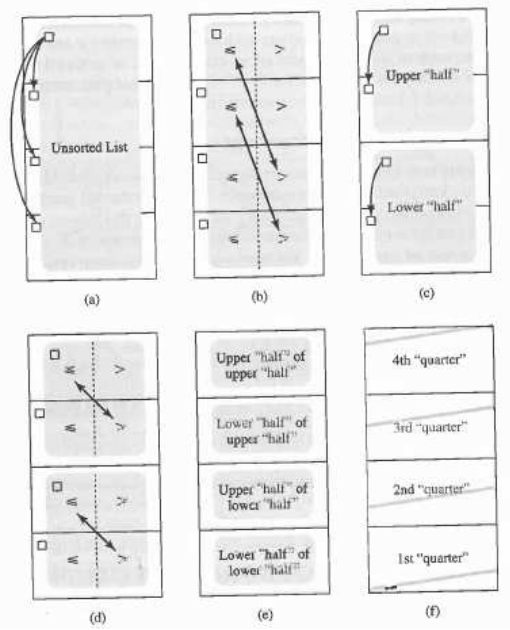
\includegraphics[height=0.4\linewidth]{Parallel_quicksort}
		\caption{Sketch of parallel quicksort}
		\label{fig:parallelquicksort}
	\end{figure}
	
	
	Sticking to this algorithm, it would only work with a number of processes which is a power of two, but with some more steps, which of course will lead more overhead, expecially when computing the algorithm with an odd number of processes, I've been able to run this process with every number of processes. I've been able to achieve this by carefully managing the odd number of processes case: in this scenario, the pivot rank will perform first its partition phase, and detect which partition has the least number of elements and scatter this partition among the corresponding halves of the processes (the left-hand side if the minor partition is the left one, and viceversa). After doing this, he will enter in the opposite communicator (the right one if the minor partition is the left one and viceversa). Then all the other processes will go on as usual.
	This introduces inevitably more overhead in the case of an odd number of processes, but makes this approach more general.
	
	\section{Result and analysis}
	
	In order to evaluate the performance of my parallel implementation, I used as main metrics 
	\begin{itemize}
		\item Time of execution;
		\item Speedup, which is provided by the formula $$Sp(N,P)=\frac{time_{serial}(N)}{time_{parallel}(N)}$$ with $N$ size of the problem and $P$ number of processes.
	\end{itemize}
	
	Each misuration was taken 5 times, and then I have considered the mean, in order to have a more robust result.
	
	\subsection{OpenMP execution time}
	
	To run this test, I've used the \textit{omp\_timings.sh} script, which takes the timings of each run by executing the program via \textit{mpirun -np 1} command, which ensures the execution by only one process, and by varying the number of threads used and mapping them by core with \textit{OMP\_PLACES=cores} and placing them close together with \textit{OMP\_PROC\_BIND=close}, making all the threads share the same L3 cache. 
	
	% INSERT PLOT RELATIVE TO TIME OF EXECUTION
	
	This plot represents the time of execution of the algorithm for a 64 million elements array for different number of threads.
	It is evident that the execution time has a diminishing trend, that however doesn't perfectly follow an inverse proportionality relation. Furthermore we can observe that the execution time tend to stall from $40$ threads on, probably due to a "starvation" effect, where there are too many threads than work to be done, and the creation and synchronization of threads take too much time with respect to the work to be done. 
	
	% Se riesci prendi tempi con più dati per vedere se cambiano i tempi
	
	This trend is even more clear when we plot the speedup graph.
	
	% INSERIRE GRAFICO SPEERDUP OMP
	
	As we can see, the OMP speedup is far from linear (a part from the up-to 4 threads scenario), and better follows a logarithmic trend. This may be due to the usage of the \textit{task} construct, where the instrucions within each construct are put in a task-scheduling list, and the first free thread takes the first available task, form a queue-like structure. This construct allows to have a static number of operating software threads decided at the beginning of the execution, but can introduce some cache related effects, as we can't manage which thread enters which task. I've tried to avoid this problem by switching to the serial algorithm if the array size fits entirely on the L1 cache of the operating threads, only marginally solving the problem.
	
	\subsection{MPI strong scalability}
	
	To run this test, I've used the \textit{smpi.sh} script, which takes the timings of each run via \textit{mpirun -np \#procs}, and mapping them by socket, minimizing, except from the first communication, the distance between operating processes, and as a consequence the time of communication. Here I've considered that each process would spawn 4 threads, which in the previous study resulted to be the most efficient number with respect to the number of elements.
	
	%INSERISCI GRAFICO TEMPISTICHE
	
	As we can see, for a sufficient large array, that would not lead to too little work assigned to each process, the trend of the timings is similar to the OpenMP case.
	However in this case there is a clearer explanation: for increasing number of processes, the number of communications increases exponentially. This allows for rapid growth of the speedup for few number of elements, but as the number of processes increases, although the workload per process is decreasing, the time taken for the communications to setup each chunk before ordering takes more and more time.
	
	% INSERISCI GRAFICO SPEEDUP
	
	As before the speedup is not lenear, but this phenomenon is explainable, as specified above, by the inclreasingly higher time taken for the communications. However the trend results to be better than the simple logarithm, expecially when the number of processes are a power of two, as the communications are balanced and reduced to the minimum.
	The generalization I've tried to assess inevitably produces some more overhead, showed by the worse speedup expecially with a prime number of processes.
	
	\subsection{MPI weak scalability}
	
	To run this test, I've used the \textit{wmpi.sh} script, which takes the timings of each run via \textit{mpirun -np \#procs}, always placing the map of the processes by socket, for the same reasons as before. I decided to keep the workload for each process constant at $240000$ elements, and set the number of threads to $4$.
	
	% INSERIRE PLOT TIMINGS
	
	As we can see, the algorithm doesn't scale perfectly when we are speaking of weak scalability, as the timings are not constant to the serial case, but we can see that for increasingly high number of processes, the timings tend to settle to a constant behavior.
	
	This is explainable by the fact that for too low number of processes, the array results to be too small to see the actual benefits of parallelism, but as the number of processes increase, yet the total size is very high, but also the time taken for communications increases with the number of processes.
	
	\section{Conclusions and further improvements}
	
	As we can see from the analysis, this implementation didn't result in an optimal linear parallelization, but it's not too surprising.
	For its nature, quicksort is not a balanced algorithm, so its purely serial part results in a huge limitation in parallelization.
	My approach focussed more on a try to carefully organize the generated data on each process, in order to then apply the serial or OMP quicksort to order each chunk. This avoids a huge roblem of a naive implementation of a parallel quicksort, which consists in:
	\begin{itemize}
		\item One process generates the data and scatters them among the processes;
		\item Each process quicksorts its chunk;
		\item Carefully merge the data back into one process.
	\end{itemize}
	This approach soffers two main issues: firstly the array we want to order may not even fit into one single node memory, but aside this, the careful merge done as last step, even though done in a binary tree fashion, results in a huge bottleneck for the computation. This way, by carefully managing the data at the beginning, we don't have to merge it into one single process, and let it scattered among processes.
	
	My solution, however, appears to be far from optimal, in a way due to the nature of the sorting algorithm, which is hardly perfectly parallelizable, and due to some improvements that could be done in the code, such as:
	\begin{itemize}
		\item Try and reduce the overhead of the algorithm when trying to select a good pivot, which consists in a gather operation followed by a sorting routine and by a scatter of the selected pivot. Maybe just randomly choosing an element from a random process and broadcast it as a global pivot could lead to less time sent in that sense, but could imply a way worse load imbalance between processes.
		\item Try and implement an algorithm that has a linear number of communication to the number of processes, such as the one referred in literature as Parallel Sorting through Regular Sampling. This approach, however, implies a prior sorting of the local chunk to select appropriate pivots and maintain load balance. This approach, however, which I had a try on implementing, resulted in way worse performance than the analyzed implementation, other than the fact that utilizing an MPI\_Alltoall operation, tends to fail with extremely high number of elements to transfer.
		\item Try and implement a similar approach also in shared memory, which would require careful threads synchronization, but would it exploit full parallelization power?
		\item Try with a different partitioning routine, for which I opted the classical serial approach, with a more parallelizable algorithm, such as Hoare partition routine.
		\item Try and organize the partitions between threads using parallel sections instead tasks. This of course could avoid some cache related effects, statically binding the recursion call to the thread, but would spawn an exponentially higher number of threads, one for each recursive call, incurring in rapid exhaustion of the threads available on the machine.
	\end{itemize}
	
	In conclusion, the solution I've come up with is hardly the best one achievable, but yet does its work to ease the computational time necessary to perform an already very efficient sorting algotithm such as quicksort on large arrays, exploiting multiple threads and processes.
	
	\newpage
	\bibliographystyle{plain}
	\bibliography{bib}
	 
\end{document}